% Skeleton for the IEEE CoG 2027 submission (Track 01, full paper, double-blind, 8 pages with references).
% Numbers in the results come from generated/numbers.tex; run `python3 docs/paper/make_results.py` first.
% Compile: pdflatex, bibtex, pdflatex, pdflatex (see README.md).
\documentclass[conference]{IEEEtran}

\usepackage[utf8]{inputenc}
\usepackage[T1]{fontenc}
\usepackage{cite}
\usepackage{amsmath}
\usepackage{booktabs}
\usepackage{graphicx}
\usepackage{textcomp}
\usepackage{url}
\usepackage{microtype}
\usepackage{tikz}
\usetikzlibrary{arrows.meta, positioning}
\usepackage{pgfplots}
\pgfplotsset{compat=1.17}

\newcommand{\AFixedMean}{56.03}
\newcommand{\ADiverseMean}{54.81}
\newcommand{\AFixedSD}{5.4}
\newcommand{\ADiverseSD}{4.9}
\newcommand{\ADelta}{$-$1.22}
\newcommand{\ACIlow}{$-$3.78}
\newcommand{\ACIhigh}{$+$1.33}
\newcommand{\ANinetyLow}{$-$3.40}
\newcommand{\ANinetyHigh}{$+$0.90}
\newcommand{\AAgreeMin}{99.8}
\newcommand{\AAgreeMax}{100.0}
\newcommand{\AAgreeFixedMean}{100.0}
\newcommand{\AAgreeDiverseMean}{100.0}
\newcommand{\ADeckGap}{16.0}
\newcommand{\AGames}{120}
\newcommand{\BFixedMean}{65.18}
\newcommand{\BDiverseMean}{66.58}
\newcommand{\BFixedSD}{3.8}
\newcommand{\BDiverseSD}{4.7}
\newcommand{\BDelta}{$+$1.40}
\newcommand{\BCIlow}{$-$0.67}
\newcommand{\BCIhigh}{$+$3.58}
\newcommand{\BNinetyLow}{$-$0.33}
\newcommand{\BNinetyHigh}{$+$3.21}
\newcommand{\BAgreeMin}{51.6}
\newcommand{\BAgreeMax}{69.3}
\newcommand{\BAgreeFixedMean}{60.8}
\newcommand{\BAgreeDiverseMean}{61.8}
\newcommand{\BDeckGap}{30.1}
\newcommand{\BGames}{120}
\newcommand{\CFixedMean}{65.76}
\newcommand{\CDiverseMean}{64.17}
\newcommand{\CFixedSD}{3.8}
\newcommand{\CDiverseSD}{4.9}
\newcommand{\CDelta}{$-$1.60}
\newcommand{\CCIlow}{$-$3.69}
\newcommand{\CCIhigh}{$+$0.61}
\newcommand{\CNinetyLow}{$-$3.40}
\newcommand{\CNinetyHigh}{$+$0.25}
\newcommand{\CDeckGap}{29.7}
\newcommand{\CGames}{120}
\newcommand{\DFixedMean}{53.92}
\newcommand{\DDiverseMean}{54.07}
\newcommand{\DFixedSD}{10.8}
\newcommand{\DDiverseSD}{10.6}
\newcommand{\DDelta}{$+$0.15}
\newcommand{\DCIlow}{$-$5.04}
\newcommand{\DCIhigh}{$+$5.29}
\newcommand{\DNinetyLow}{$-$4.29}
\newcommand{\DNinetyHigh}{$+$4.51}
\newcommand{\DDeckGap}{5.9}
\newcommand{\DGames}{120}
\newcommand{\SDMin}{3.8}
\newcommand{\SDMax}{10.8}
\newcommand{\MaxBound}{5.29}
\newcommand{\MaxDelta}{1.60}
\newcommand{\AuditGames}{300}
\newcommand{\AuditSnorlaxNoPokemon}{266}
\newcommand{\AuditSnorlaxPrizes}{34}
\newcommand{\AuditSnorlaxMedian}{12}
\newcommand{\AuditMewtwoDeckOut}{205}
\newcommand{\AuditMewtwoPrizes}{89}
\newcommand{\AuditMewtwoMedian}{57}
\newcommand{\CChangeFixed}{$+$0.6}
\newcommand{\CChangeFixedSD}{5.1}
\newcommand{\CUpFixed}{17}
\newcommand{\CTrainFirstFixed}{58.0}
\newcommand{\CTrainLastFixed}{57.9}
\newcommand{\CChangeDiverse}{$-$1.0}
\newcommand{\CChangeDiverseSD}{5.9}
\newcommand{\CUpDiverse}{11}
\newcommand{\CTrainFirstDiverse}{69.4}
\newcommand{\CTrainLastDiverse}{69.7}
\newcommand{\StartMean}{65.18}
\newcommand{\DTrainFirstFixed}{44.7}
\newcommand{\DTrainLastFixed}{49.9}
\newcommand{\DUpFixed}{25}
\newcommand{\DTrainFirstDiverse}{54.5}
\newcommand{\DTrainLastDiverse}{63.2}
\newcommand{\DUpDiverse}{25}
\newcommand{\DMewtwoGap}{$-$6.4}
\newcommand{\DMewtwoGapLow}{$-$13.9}
\newcommand{\DMewtwoGapHigh}{$+$1.2}
\newcommand{\DSnorlaxGap}{$+$6.8}
\newcommand{\DSnorlaxGapLow}{$-$2.2}
\newcommand{\DSnorlaxGapHigh}{$+$15.7}

\newcommand{\todo}[1]{\textbf{[TODO: #1]}}

\begin{document}

\title{Does the Training Opponent Matter? Four Preregistered Studies of a Compact Pok\'emon Card Game Policy}

\author{\IEEEauthorblockN{Anonymous Authors}
\IEEEauthorblockA{Submitted for double-blind review}}

\maketitle

\begin{abstract}
Agents for collectible card games are often trained against a single opponent, and a more varied set of opponents is expected to generalize better to unseen decks. We test this for a 2,881-parameter option-scoring policy in the Pok\'emon Trading Card Game environment CABT, on deck families held out from training. Four preregistered studies, each with 30 training seeds per arm and 7,200 held-out games, compare a fixed opponent pool with a diverse one. In two studies the policy imitates a rule-based teacher whose demonstrations are collected against each pool. In the other two it learns from its own wins and losses. The difference in held-out win rate is \ADelta, \BDelta, \CDelta{} and \DDelta{} points, and the 90\% interval of each difference lies inside the preregistered margin of five points. The first study could not have found an effect: the student copied its teacher on at least \AAgreeMin\% of held-out decisions. With a teacher that reads the board, agreement falls to about 61\% and the pools remain equivalent. Learning from play moved the policies by about the size of evaluation noise at 400 games and learned clearly at 2,000 games from random weights, where the margin is met only just. Both budgets are far below those of competition entries.
\end{abstract}

\begin{IEEEkeywords}
Pok\'emon Trading Card Game, imitation learning, opponent diversity, equivalence testing, preregistration
\end{IEEEkeywords}

\section{Introduction}

Collectible card games combine hidden information, a large and changing set of legal actions, and decks that change what good play looks like. Work on competition-level agents trains them against populations of opponents, and several authors argue that the variety of opponents seen in training determines how far an agent generalizes \cite{Lanctot17,Strouse21}. For small agents that must run within a fixed inference budget, it is cheaper to ask whether such variety pays off before building a population.

We ask one question: does the set of opponents used during training change a compact policy's win rate on decks it never saw? The policy is a 2,881-parameter network that scores the legal options at each decision in the Pok\'emon Trading Card Game environment CABT \cite{cabt}. We test two ways a pool of opponents can enter training. In imitation, the pool only decides which game states a teacher visits while its decisions are recorded. In learning from play, the pool supplies the wins and losses the policy learns from.

We make three contributions.
\begin{enumerate}
  \item A preregistered protocol for small studies in CABT: the plan is frozen before the run, the training seed is the unit of analysis, intervals come from a cluster bootstrap, and a margin of five points is fixed in advance so that a null result can be stated with a bound.
  \item Four controlled comparisons, each with 30 seeds per arm, that find the fixed and diverse pools equivalent within that margin.
  \item An account of why the first comparison was forced, and a second teacher that removes the cause. We also state where the learning-from-play comparisons are limited.
\end{enumerate}
We searched arXiv and the public write-ups of the 2026 competition and found no earlier controlled test of this question, for imitation learning or for card games.

\section{Related work}

\textbf{Card games as a testbed.} Collectible card games combine hidden information with a branching factor that changes with the game state and is often large. Hoover et al.\ \cite{Hoover19} note that these games are relatively understudied in AI research despite their popularity, and lay out the challenges Hearthstone poses. For a competition-level agent, Xi et al.\ \cite{Xi23} describe an end-to-end policy and an optimistic smooth fictitious play method for Legends of Code and Magic, and report winning both the official LoCM 1.5 track and the bonus LoCM 1.2 track of the COG 2022 competition. The Pok\'emon Trading Card Game has received less attention. PTCG-Bench \cite{Hua26} evaluates large language model agents on it. The 2026 Kaggle Pok\'emon TCG AI Battle, run on the same CABT engine, produced public write-ups from many learned agents. Several top entries trained by reinforcement learning from self-play or against a league of frozen opponents \cite{Kaggle7th,Kaggle6th}. One team distilled a gradient-boosted teacher into a network and notes that the teacher's games widen the training states but inherit the teacher's weaknesses \cite{Kaggle24th}. Another reports that every hand-written rule or mechanical teacher it tested cost win rate \cite{Kaggle7th}. We study a different agent class, a 2,881-parameter option scorer that runs in well under a millisecond, and we test the opponent pool directly.

\textbf{Opponent diversity and generalization.} Lanctot et al.\ \cite{Lanctot17} show that policies learned by independent reinforcement learning can overfit to the policies of the other agents seen in training, and propose best responses to mixtures of policies. Strouse et al.\ \cite{Strouse21} argue that a diverse set of training partners is the crux of generalizing to new partners in cooperative play. Both train by reinforcement learning from play, as our studies C and D do. In the first two, the opponent affects only which states the demonstrations visit. For generalization more broadly, Cobbe et al.\ \cite{Cobbe19} separate training and test sets of procedurally generated environments, and Kirk et al.\ \cite{Kirk23} survey zero-shot generalization. In the competitive Pok\'emon video game, VGC-Bench \cite{Angliss26} provides behavior cloning and self-play baselines and reports that, as the number of team configurations grows, the best single-team algorithm does worse and is more exploitable but generalizes better to unseen teams. We follow the practice of keeping the test deck families out of training, with a disjointness check between the splits.

\textbf{Imitation under distribution shift.} The learner's own mistakes lead it to states the demonstrator did not visit, which breaks the assumption of identically distributed data. Ross et al.\ \cite{Ross11} describe this compounding of errors and propose DAgger, which gathers trajectories with the current learned policy. DART \cite{Laskey17} instead injects noise into the supervisor while it demonstrates, so that the demonstrations cover recoveries. Belkhale et al.\ \cite{Belkhale23} formalize data quality through distribution shift and show that state diversity is not always beneficial and that its effect depends on action divergence and transition diversity. Our first two studies vary the demonstration states in a similar way, through the opponent, and the teacher agreement we report measures how close the learner stays to the demonstrator.

\textbf{Statistical practice.} Henderson et al.\ \cite{Henderson18} document how environment non-determinism and variance in the methods make reinforcement learning results hard to interpret without significance measures. Agarwal et al.\ \cite{Agarwal21} show that point estimates from a few training runs can mislead and recommend interval estimates. The CABT engine shuffles with a system entropy source, so no game can be replayed from a seed. We therefore treat the training seed as the unit and fix the analysis before each run.

\section{Environment, policy and agents}

\textbf{Environment.} We use CABT 1.0.0 through kaggle-environments 1.33.0 \cite{cabt,kaggleenv}, with its 1,431-card catalog pinned by SHA-256 hash. An agent receives only its own observation, with the opponent's hand masked, and returns the indices of the options it chooses. The engine seeds its shuffles from the system entropy source, so games are not replayable from seeds and we keep a record of every game instead.

\textbf{Policy.} The policy is a two-layer network, 88 inputs to 32 hidden units to one logit, with 2,881 parameters, written in NumPy. The 88 inputs are 72 features of the board (turn, prizes, hand and deck sizes, HP, attached energy and status for the active Pok\'emon and five bench slots of both sides) and 16 features of one option (its CABT option type, attack damage, whether it targets the active Pok\'emon or the bench, and its position in the list). The network scores every legal option, and the policy plays the highest score at test time.

\textbf{Teachers.} \emph{HeuristicAgent} ranks options by type and attack damage: attacks first, then attaching, evolving, playing a card and ending the turn. It never reads the board. \emph{BoardAgent} reads it. It takes a knockout when one is on offer, evolves, keeps two Pok\'emon on the bench, attaches energy where it brings an attack closest, retreats an active Pok\'emon that cannot attack or would be knocked out next turn, and values searched and discarded cards by the board. It uses only its own observation and the public card catalog.

\textbf{Decks and opponents.} Each deck family has 4 + 4 Pok\'emon, 4 + 4 Trainers and 44 basic Energy cards. The training families are water-kyogre, grass-bulbasaur and lightning-pikachu. The held-out families are psychic-mewtwo and colorless-snorlax, and every evaluation game is a mirror match. A tuning family, fire-ponyta, was used only in the pilot for study C. The \emph{fixed} pool is the engine's first-option agent in every training game. The \emph{diverse} pool draws the heuristic, the first-option agent or a random agent at each game. The same three agents are the evaluation opponents, so the held-out axis is decks and not opponents.

\begin{figure}[t]
\centering
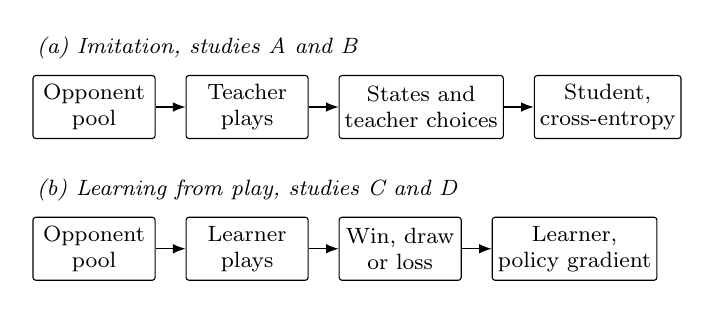
\begin{tikzpicture}[font=\footnotesize,
  box/.style={draw, rounded corners=1pt, minimum height=0.8cm, minimum width=1.55cm, align=center, inner sep=2pt},
  arr/.style={-{Latex[length=1.6mm]}}]
  \node[font=\footnotesize\itshape, anchor=west] (la) at (0,1.65) {(a) Imitation, studies A and B};
  \node[box] (p1) at (0.85,0.9) {Opponent\\pool};
  \node[box, right=0.38cm of p1] (t) {Teacher\\plays};
  \node[box, right=0.38cm of t] (d) {States and\\teacher choices};
  \node[box, right=0.38cm of d] (s) {Student,\\cross-entropy};
  \draw[arr] (p1)--(t); \draw[arr] (t)--(d); \draw[arr] (d)--(s);
  \node[font=\footnotesize\itshape, anchor=west] (lb) at (0,-0.15) {(b) Learning from play, studies C and D};
  \node[box] (p2) at (0.85,-0.9) {Opponent\\pool};
  \node[box, right=0.38cm of p2] (l) {Learner\\plays};
  \node[box, right=0.38cm of l] (o) {Win, draw\\or loss};
  \node[box, right=0.38cm of o] (u) {Learner,\\policy gradient};
  \draw[arr] (p2)--(l); \draw[arr] (l)--(o); \draw[arr] (o)--(u);
\end{tikzpicture}
\caption{Where the opponent pool acts. In imitation it decides which states the teacher visits. In learning from play it supplies the outcomes the policy learns from.}
\label{fig:pool}
\end{figure}

\section{Studies and statistics}

Table~\ref{tab:design} lists the four studies. Each has a plan frozen before its run, in machine-readable form that the runner refuses to execute unless it is marked frozen. Both arms of a study share the architecture, budget, decks and evaluation, so the pool is the only difference.

\begin{table}[t]
\caption{The four studies. Each has 30 training seeds per arm.}
\label{tab:design}
\centering
\small
\setlength{\tabcolsep}{4pt}
\begin{tabular}{@{}lllll@{}}
\toprule
 & Learner & Teacher & Start & Budget per checkpoint \\
\midrule
A & imitation & heuristic & random & 2,000 decisions, 400 steps \\
B & imitation & board & random & 2,000 decisions, 400 steps \\
C & REINFORCE & none & study B & 400 games, 50 updates \\
D & REINFORCE & none & random & 2,000 games, 250 updates \\
\bottomrule
\end{tabular}
\end{table}

\textbf{Imitation (A and B).} The teacher plays one of three training decks against the pool, and its first choice at each decision with more than one option becomes a training example. Each checkpoint trains on 2,000 decisions (1,600 for training and 400 for validation) for 400 Adam steps.

\textbf{Learning from play (C and D).} The policy samples each choice from the softmax of its option scores, plays a full game against the pool from a random seat and deck, and receives $+1$, $0$ or $-1$ for a win, draw or loss. REINFORCE updates it after every batch of 8 games with the batch mean outcome as the baseline and Adam at learning rate 0.003, for 400 games. Both arms start from the board-teacher checkpoint of the same seed, so the pool is again the only difference. A pilot chose the learning rate from 0.001, 0.003 and 0.01. It used four seeds outside the study and scored 60 games per checkpoint on the tuning deck. At 0.003 the pilot gained 11.7 points (fixed pool) and 5.0 (diverse pool) over the starting checkpoints, and the other two rates gained about nothing. On the held-out decks the gain did not carry over (Section~\ref{sec:results}), so the pilot was too small to select a rate reliably. Study D gives learning more room: the policy starts from random weights and plays 2,000 games (250 updates) at learning rate 0.03. An 800-game pilot from the imitation start (two seeds per arm) had found no learning at any of the three rates, and a pilot from random weights was the only one in which training scores rose, at 0.03. The plan for D records that the design changed after the pilots and before any study game.

\textbf{Evaluation.} Each checkpoint plays 120 held-out games: 2 decks $\times$ 3 opponents $\times$ 5 evaluation seeds $\times$ 2 pairs, with seats reversed inside each pair. A draw counts as half a win. The checkpoint score is the mean of its win rates on the two held-out decks.

\textbf{Statistics.} The unit is the training seed. The estimate is the mean checkpoint score of the diverse arm minus that of the fixed arm. The interval is a percentile cluster bootstrap that resamples seeds within each arm, with 10,000 resamples. A difference is reported when the 95\% interval excludes zero. Equivalence is reported when the 90\% interval lies inside $\pm 5$ points, the bootstrap form of two one-sided tests at the 5\% level. Otherwise the result is inconclusive. The margin was chosen before any data, at less than half the 12-point gap between the two held-out decks in an earlier run.

\section{Results}
\label{sec:results}

\begin{table*}[t]
\caption{Difference in held-out win rate, diverse minus fixed pool, in percentage points. Means are checkpoint scores over 30 seeds per arm. Intervals are cluster-bootstrap intervals over training seeds. Equivalence uses the margin of $\pm 5$ points.}
\label{tab:results}
\centering
\small
\begin{tabular}{@{}lrrrccl@{}}
\toprule
Study & Fixed mean (\%) & Diverse mean (\%) & Difference & 95\% interval & 90\% interval & Result \\
\midrule
A & 56.03 & 54.81 & $-$1.22 & [$-$3.78, $+$1.33] & [$-$3.40, $+$0.90] & equivalent \\
B & 65.18 & 66.58 & $+$1.40 & [$-$0.67, $+$3.58] & [$-$0.33, $+$3.21] & equivalent \\
C & 65.76 & 64.17 & $-$1.60 & [$-$3.69, $+$0.61] & [$-$3.40, $+$0.25] & equivalent \\
\bottomrule
\end{tabular}

\end{table*}

Table~\ref{tab:results} gives the preregistered result. In all four studies the 95\% interval includes zero and the 90\% interval lies inside the margin, so the pools are equivalent within five points. Fig.~\ref{fig:seeds} shows every seed. The standard deviation across seeds inside one arm is \SDMin{} to \SDMax{} points, larger than every difference.

\begin{figure}[t]
\centering
\begin{tikzpicture}
\begin{axis}[width=\columnwidth, height=5.2cm, ymin=40, ymax=80, xmin=0.3, xmax=11.7,
  xtick={1,2,4,5,7,8,10,11}, xticklabels={fix,div,fix,div,fix,div,fix,div},
  ylabel={Held-out win rate (\%)}, ylabel style={font=\footnotesize},
  tick label style={font=\footnotesize}, ymajorgrids, grid style={black!12}, clip=true]
  \addplot[only marks, mark=o, mark size=1.1pt, draw=black!70] table[col sep=comma, x=x, y=score] {generated/seed-scores-fixed.csv};
  \addplot[only marks, mark=triangle*, mark size=1.2pt, draw=black!70, fill=black!70] table[col sep=comma, x=x, y=score] {generated/seed-scores-diverse.csv};
  \addplot[only marks, mark=-, mark size=6pt, very thick, draw=black] table[col sep=comma, x=x, y=mean] {generated/arm-means.csv};
  \node[font=\footnotesize] at (axis cs:1.5,41.8) {A};
  \node[font=\footnotesize] at (axis cs:4.5,41.8) {B};
  \node[font=\footnotesize] at (axis cs:7.5,41.8) {C};
  \node[font=\footnotesize] at (axis cs:10.5,41.8) {D};
\end{axis}
\end{tikzpicture}
\caption{Held-out win rate of every checkpoint. Fix is the fixed pool (open circles), div the diverse pool (filled triangles), and the bar is the arm mean. A and B imitate a heuristic and a board-reading teacher, and C and D learn from play (C from the imitation checkpoints, D from random weights). Points are spread sideways by seed order only.}
\label{fig:seeds}
\end{figure}

\textbf{Study A was forced.} The students matched the heuristic teacher on \AAgreeMin\% to \AAgreeMax\% of held-out decisions with more than one option. The heuristic scores an option by its type and damage, and the student's features hold both, so any demonstrations teach the same rule and the pool has nothing to change. Study A therefore says little about the pool. We built study B to remove this cause.

\textbf{Study B.} With the board-reading teacher the students agree with it on \BAgreeMin\% to \BAgreeMax\% of held-out decisions (mean \BAgreeFixedMean\% for the fixed arm and \BAgreeDiverseMean\% for the diverse arm). They no longer copy the teacher, and the pools are still equivalent: the difference is \BDelta{} points with a 95\% interval of [\BCIlow, \BCIhigh]. This is the main result of the paper.

\textbf{Study C.} Learning from play moved the policies very little. Against the checkpoint each seed started from (mean score \StartMean\%), the change was \CChangeFixed{} points for the fixed arm (\CUpFixed{} of 30 seeds up) and \CChangeDiverse{} for the diverse arm (\CUpDiverse{} of 30), with a standard deviation of \CChangeFixedSD{} and \CChangeDiverseSD{} points. A 120-game score alone has a standard error near 4.5 points, so these changes are about the size of evaluation noise. The mean training score also stayed flat, from \CTrainFirstFixed\% to \CTrainLastFixed\% for the fixed arm and \CTrainFirstDiverse\% to \CTrainLastDiverse\% for the diverse arm. The equivalence in C is therefore weak evidence about the pool. It shows no effect at a budget of 400 games, and does not show that learning from play is unaffected by its opponents. Study D gives learning more room.

\textbf{Study D.} With 2,000 games from random weights the policies learned. The mean training score rose from \DTrainFirstFixed\% to \DTrainLastFixed\% for the fixed arm and from \DTrainFirstDiverse\% to \DTrainLastDiverse\% for the diverse arm, and it rose in \DUpFixed{} and \DUpDiverse{} of 30 seeds. The held-out scores, \DFixedMean\% and \DDiverseMean\%, are below the imitation students of study B and close to the heuristic. The seed-to-seed spread is about 10.6 points, more than twice that of the imitation studies. The 90\% interval, [\DNinetyLow, \DNinetyHigh], lies inside the margin with little room, and a margin below 4.5 points would have left the result inconclusive. As an unplanned observation, the arms differ by deck in opposite directions: \DMewtwoGap{} points on psychic-mewtwo (95\% interval [\DMewtwoGapLow, \DMewtwoGapHigh]) and \DSnorlaxGap{} on colorless-snorlax ([\DSnorlaxGapLow, \DSnorlaxGapHigh]). Both intervals include zero, and the two gaps cancel in the primary score.

\textbf{Decks and opponents.} Table~\ref{tab:split} splits the win rates by held-out deck and by evaluation opponent. The deck matters far more than the pool. Averaged over the two arms, the colorless-snorlax deck scores \ADeckGap, \BDeckGap, \CDeckGap{} and \DDeckGap{} points above psychic-mewtwo in studies A to D, against pool differences of at most \MaxDelta{} points. With two held-out decks, a deck effect cannot be separated from deck-specific play, and we do not model it.

\begin{table}[t]
\caption{Mean win rate (\%) by held-out deck and by evaluation opponent, over 30 seeds per arm.}
\label{tab:split}
\centering
\small
\setlength{\tabcolsep}{3.5pt}
\begin{tabular}{@{}llrrrrr@{}}
\toprule
 & & \multicolumn{2}{c}{Held-out deck} & \multicolumn{3}{c}{Opponent} \\
\cmidrule(lr){3-4}\cmidrule(lr){5-7}
Study & Arm & Mewtwo & Snorlax & Heuristic & First & Random \\
\midrule
A & fixed & 48.3 & 63.7 & 48.5 & 58.3 & 61.3 \\
A & diverse & 46.5 & 63.1 & 48.5 & 56.5 & 59.3 \\
B & fixed & 49.9 & 80.4 & 59.3 & 66.2 & 70.0 \\
B & diverse & 51.7 & 81.4 & 61.9 & 66.0 & 71.9 \\
C & fixed & 50.5 & 81.0 & 62.0 & 67.9 & 67.4 \\
C & diverse & 49.7 & 78.6 & 58.5 & 66.1 & 67.9 \\
\bottomrule
\end{tabular}

\end{table}

\textbf{Baselines.} Table~\ref{tab:baselines} gives four reference agents under the same 120-game protocol. Win rates for the same agent differ by up to 8 points between studies, which shows how noisy 120 games are. Students in studies B and C score between the board teacher and the other three agents, and the learned policies of study D score near the heuristic.

\begin{table}[t]
\caption{Win rate (\%) of reference agents on the held-out decks, 120 games each, same protocol as the students. Study A did not include the board agent.}
\label{tab:baselines}
\centering
\small
\begin{tabular}{@{}lrrrr@{}}
\toprule
Study & Board & Heuristic & First & Random \\
\midrule
A & n/a & 56.7 & 39.6 & 41.7 \\
B & 74.6 & 58.3 & 52.1 & 53.8 \\
C & 75.0 & 57.1 & 45.4 & 50.4 \\
D & 70.4 & 53.8 & 49.2 & 44.2 \\
\bottomrule
\end{tabular}

\end{table}

\section{Discussion}

The pool did not change held-out play in any of the four designs, within five points. We see three readings, and the data do not separate them. First, in imitation the pool changes only which states the teacher visits, and the teacher's choice is a function of the state, so a student that fits the teacher well on any reasonable sample of states ends up close to the same function. Second, in learning from play, the budget may be too small for the opponent to matter. Study D raised it fivefold, from random weights, and found the same, but 2,000 games is far below the roughly 20 million used by one competition entry \cite{Kaggle20th}. Third, the evaluation opponents are the same three agent types as the diverse pool, so the diverse pool is not out of distribution at test time. The comparison asks about unseen decks only.

\textbf{Study history.} The studies were not our first runs. Earlier three-seed runs of study A gave differences of $-3.88$ (not logged), $-0.55$ and $+6.95$ points. The last came after we fixed a defect in which the teacher always played the water-kyogre deck whatever the training deck. The 30-seed run gave \ADelta{} points. The seed-level analysis and the preregistered plans followed from that spread. Study A also used a feature encoder whose bench flag never fired, which we corrected before studies B and C. The pilots for studies C and D used seeds outside the studies.

\section{Limitations}

\begin{itemize}
  \item The decks are simplified and every held-out game is a mirror match. The 30-seed reports do not store replays, so we measured end reasons in a separate audit of 600 games: four study B checkpoints (seeds 2001 and 2002, both arms) and the board teacher, 120 games each, which gives \AuditGames{} games per deck. On colorless-snorlax, \AuditSnorlaxNoPokemon{} of \AuditGames{} games ended with a player having no Pok\'emon left, with a median of \AuditSnorlaxMedian{} turns. On psychic-mewtwo, \AuditMewtwoDeckOut{} ended by deck-out, with a median of \AuditMewtwoMedian{} turns. Only \AuditSnorlaxPrizes{} and \AuditMewtwoPrizes{} games on the two decks ended by taking all prize cards, the usual way to win, so most games end by another route.
  \item The margin of five points is a judgment, and a reviewer may prefer another. The 95\% intervals rule out differences larger than \MaxBound{} points in all four studies, and say nothing about smaller ones. In study D the 90\% interval fits inside the margin with little room.
  \item Studies C and D used small budgets and learning rates chosen in pilots of two to four seeds on one deck. Study C started both arms from an imitation checkpoint, and study D learned from random weights and reached only about the strength of the heuristic. Neither speaks to a budget in the millions of games.
  \item One architecture and one environment were used, with three simple opponents. Nothing here is evidence about population training at the scale of the competition entries.
  \item The study measures win rate against three fixed agents. It does not measure exploitability or play against humans.
\end{itemize}

\section{Conclusion}

Across four preregistered designs, training against a diverse opponent pool did not change a compact policy's win rate on unseen decks by more than about five points. The first design could not have shown an effect, the second removes that cause, the third is limited by a small budget, and the fourth lets learning from random weights run for 2,000 games and still finds no effect, though only just inside the margin. A stronger test of learning from play needs far more games per checkpoint than we could run.

\textbf{Reproducibility.} Plans, reports, checkpoints and code are available at \todo{anonymized link for review; public link after acceptance}. The CABT engine cannot replay games from seeds, so the per-game records in the reports are the record of every game.

\bibliographystyle{ieee/IEEEtran}
\bibliography{refs}

\end{document}
